\documentclass{article}
\author{Trever Hallock}
\title{A Genetic Algorithm for finding efficient representations of Pareto Optimal Sets}

\usepackage{graphicx} 

\begin{document}
\maketitle


\begin{abstract}
Random sampling can be effective to solve multi-objective problems not with standing their complete lack sophistication.
This begs for an algorithm that can harness the advantages of random point generation while improving the generation process.
This paper describes how to use a genetic algorithm to smartly guide how new random points are chosen.
\end{abstract}

\pagebreak


\section{Introduction}

The purpose of this paper is present a genetic algorithm for solving multi-objective optimization problems.
A multi-objective optimization problem is the problem of minimizing $f(x)$ s.t. $x \in X$ for some vector-valued function $f:R^n \Rightarrow R^p$.
The set $X$ is called the feasible region, or decision space, while $f(X)$ is the outcome space.
Because $f$ is vector-valued, there will not generally be a single optimal solution but several outcomes that are not clearly better than each other.
This is true when different components of $f$ (which can be thought of as different objectives) are competing with each other, so that different ``good" points may represent trade-offs between the $p$ 
different components.
To describe the set of equally optimal points, we say an outcome $f(x_1)$ is said to dominate another $f(x_2)$ if $f(x_1)_i \le f(x_2)_i, i=1,2, ..., p$ and $\exists i$ s.t. $f(x_1)_i < f(x_2)_i$.
Then the optimal set of points is defined to be those outcomes $y = f(x)$ for which there exists no $x'$ such that $f(x')$ dominates $f(x)$.
This set is called the pareto optimal set, and the $x$ values that produce the pareto optimal set are called efficient.

A multi-objective solver is an algorithm that accepts an $f$ and some representation of a feasible region to produces a representation of the pareto optimal set.
This paper is concerned with designing an evolutionary solver, which will find the representation by modelling evolutionary principles to evolve an initial random sample.
The representation created is simply a set of points called a population that belong to the pareto set, and each member of the representation is called an individual.
The evolutionary principles include a selection mechanism based on some measure of the fitness of individuals to steer the population towards a ``good" representation.
They include a cross over function that is used to generate new individuals (called offspring) from the existing population, as well as mutation of the offspring
to diversify the population and potentially discover new regions of the pareto set.


\section{Motivation}

Randomly sampling the feasible region and simply using the generated $f$ values works remarkably well.
After comparing several solvers on a test set of problems in class (from problem set 1),
the random sampler was not only consistently very fast, but usually did a good job of finding each disconnected pareto optimal region.
Although this was slightly disappointing considering the effort that went into the other solvers, it does motivate basing an algorithm on random point generation with
the expectation that should be many \emph{simple} ways of improving random sampling.

One approach that improves uniformly sampling the feasible region is moving the expected value of a random sample generator towards the pareto frontier as well as adapting the
distribution's expected variation as the frontier is more densely enumerated.
However, it seems that evolutionary computation should do even better, because the advantages random point generation should be reproducible in a genetic algorithm through the mutation process.
Although the genetic algorithm may incur additional runtime costs from crossover or selection, the complexity involved with these operations can be limited
base on how helpful they are in improving the sample.

I was also interested in this topic because I haven't written many genetic algorithms, and I was interested in learning the concepts terminology from the field.
Out of the different multi-objective related projects, this application seemed to be a useful, computational route.

\section{Criteria for the Algorithm}

Before we develop the algorithm, we must know how to evaluate the efficiency of the algorithm itself, and
there are many ways to measure how well a multi-objective solver performs.
We will consider the solver's performance, completeness, and generality.

The \emph{generality} describes what problems the solver is able to solve.
For example, an algorithm may only solve convex problems, connected pareto solutions, or place other assumptions on how to express the feasible set.
For example, Matlab's genetic algorithm \emph{gamultiobj} assumes that the feasible region is the set of $x$ satisfying $Ax = b$, $Ax \le b$, or $b_1 < x < b_2$ for some input $A, b, b_1, b_2$.

The algorithm I develop is designed to solve any multi-objective problem that is bounded in the decision space, and bounded below in the outcome space.
An arbitrary, boolean-valued function is passed to algorithm to characterize the feasible region within the bounds (which are passed as an upper and lower bound containing the feasible region as a subset).
These constraints are currently in place to aid in random point generation, although it may be possible to generalize this by providing a generator that maps to more general feasible regions.
(Although continuity is not strictly required, the algorithm works by assuming breeding optimal points with those other fit points,
so there is some assumption of optimal points being close to other optimal points)

Defining the \emph{completeness} of the algorithm will be an important concern of this project.
This measures how well the outcome set represents the entire pareto-optimal set.
To motivate the later discussion, the output set should be \emph{efficient} in that each point contributes information about the optimal set without duplicating another point.
It should also be \emph{entire} in that it should ideally contain points in most if not all disconnected feasible regions when possible, and it should somehow spread out over these regions.
It should also be meaningful, which means it can't be too big or too small.
When a set is complete, we would expect that by minimizing/maximizing each component of all optimal points will accurately describe both the ideal point and the nadir point.


The \emph{performance} of the algorithm should describe how long the algorithm takes to run.
In many cases this is described by the order of the asymptotic runtime.
However, one of the inputs to the algorithm is the function that needs to be optimized, which can be arbitrarily complicated.
This means that the preferred measure of runtime is in the number of objective-function evaluations.
Of course, we can still consider the overall runtime of the algorithm itself, as an inordinately long runtime will limit the algorithm's applicability to simple problems.


Although we will explain these in more detail, these considerations inspired my first, primitive metric.
According to these thoughts, the preliminary bi-criteria the optimization problem was to select the algorithm that maximized the
pair $(y_N - y_I, |S|)$ where $y_{Ni} = \max y_i $ and $y_{Ii} = \min y_i$ for all $y \in S$ where $S$ is the set of pareto points found by the algorithm.
We will later discuss improvements to this, for example this in no way penalizes duplicate points and potentially only encourages only $2$ diverse points.
(For example, on the bi-criteria optimization problem with a one dimensional pareto set $y_2 = 1-y_1$ from $(1,0)$ to $(0,1)$, the set with $x$ values of $(0, 4.999, .5, .5001, 1)$
would be just as good as one that produces $x$-values of $(0, .25,  .5, .75 ,1)$.)


\section{Representational Quality}

With these criteria, one significant subproblem is as follows.
Either at completion of the algorithm, or potentially to guide it as it is still running, the algorithm 
will have a set of vector-pairs $S \subset \{(x,y) | y = f(x)\}$ for which the objective values have already been computed and will need to find a subset
$R$ of $Y(S) = \{y | (x,y) \in S\}$ that best represents the true pareto set.
Of course, the pareto set will not be available to the algorithm, so that it will need to approximate the final set with the points it already knows.

To solve this problem, we have to be able to compare how well different subsets represent the pareto set, as well as be able to efficiently find those representations that are best.
In small dimensional cases, the best representation should agree with what we visually (or intuitively) feel is the best representation.
It should also be reasonably efficient to compute.
I will consider a couple different metrics, and decide which works the best.
We can adapt an approach taken in [citation here] where this problem is presented as a tri-criteria optimization problem.

One dimension is $\delta = \max_{y} \min_{y'} d(y, y')$ for each $y, y' \in Y(S)$ s.t. $y \ne y'$.
We will discuss which metric $d$ to use later.
This dimension should be minimized, because a large value means that some points are isolated.
This quantity is the farthest distance from any point to its closest neighbor.
This is an attempt at approximating how far any possible point in the outcome space is from a point in the representation.
Because this only looks at the closest point to any given point, it does have significant draw backs.
For example, if the $y$'s are the following set $(0, .01, .98, .99, 1)$ which are supposed to represent the interval from $[0,1]$.
Each point has a neighbor that is within $.01$ of itself while there still seems to be a large gap in the set.
Spreading out these points more evenly would even hurt metric.
This brings out that this measure suffers when the $Y(S)$ only poorly represents the entire space before we even start taking subsets.

It also makes it clear that as it is more meaningful when $|R| \ll |S|$ and with constraints that $y' \in R$.
We would hope this means that several points within the gap would introduce penalties around $.97$ for this representation.
%This brings out that this measure fails when $Y(S)$ is a bad representation of the pareto set before we even start taking subsets.
In this example, another improvement may be to average the $k$ closest points.
If we took $k = 2$, then each point but $1$ would be penalized by the the second closest point.
One might could use weights to account for the bias this would induce when several points are clustered.
For example, consider a $Y(S)$ with many points tightly clustered around $0$ with few equally spaced point out to $1$.
Then as $k$ grows large (say close to $|Y(S)|$), the cluster will pull the representation towards its center as these points will have the least summed distance to all other points.
The resulting measure would look like this:
$$\sum_y \sum_{i=0}^k (y  )( closest(y, i) )( w_{closest(y, i)})$$
with $closest(y,i)$ being the $i$th closest point to $y$, and $w_y$ being a weight assigned to each point.
Likely the $w_i$ will not need to vary from $1$ unless $k$ is large and $S$ is skewed.
In this case they should be smaller for points in a dense area of $S$.


Another dimension is $\epsilon = \min_{y,y'} d(y,y')$.
This component is to be maximized, because when it is small, the representation contains duplication.
Of course, this could also include the distance from any given point to multiple other points to improve its robustness.
For example, a set that is nearly perfect except two points that happen to be very close will suffer under this metric.
If this were instead the average of all $d(y, closest(y))$ for all $y \in R$, it may coincide with our expectations better.

Finally, the paper considers $|R|$ which is to be minimized.
In general, this is expected to be a ``reasonable" number for the size of the pareto set.
For several purposes, it will be useful to simply specify a $|R|$.
That is, the problem statement will be to find the best representation in term of the diversity/duplication for a given number of points.


While comparing different measures of how good the representation is, the algorithm will also need to find them efficiently.
The first implementation I wrote is a simple backtracking algorithm described by the following pseudo code.
It enumerates all subsets of $Y(S)$ by recursing on the number of points that are determined to be in the set or out.
It creates a mask representing the subset, so that the different measures (passed as ``metric" to the algorithm) will simply take in the original set and a mask of which points to include.


\begin{verbatim}
backtrack (int num_determined, boolean[] mask, metric, S)
{
	if num_determined = |S|
	{
		candidate := metric ( S , mask )
		if candidate is not pareto optimal
		{
		  return
		}
		
		add candiate to set of pareto subsets
		remove any subsets dominated by candidate
		return
	}
	
	mask[num_determined] = 0
	backtrack(point + 1, mask, metric, S)
	
	mask[num_determined] = 1
	backtrack(point + 1, mask, metric, S)
}

solve ( S , metric)
{
      backtrack( 0 , new mask[], metric, S)
}
\end{verbatim}


This has $2^{|S|}$ time complexity so it is not computationally practical unless either $|S| < 30$ or bounds are provided for $\epsilon$ and $\delta$ to prune branches early.
For example, a lower bound on $\epsilon$ removes the branch with mask[num determined] = 1 for any points that are closer to the num determined point.
In order to consider all possible points, the algorithm would also need to backtrack on the order of removing close points that violate the $\epsilon$ constraint.
Although the constraint that the number $|R|$ of points in the representation be a given value could be included into this algorithm, 
there are many faster techniques for enumerating all ${|S|} \choose {|R|}$ such subsets.

This problem may also be quickly solvable with a genetic algorithm.
If the best representation, or at least a good one is computed repeatedly as a selection process for the outer algorithm, then perhaps fewer generations will have to be used.
This is because the net affect of each step accrues at each later generation.
The inner genetic algorithm is very similar to the outer, and could be seen as simply an extension of the evolutionary model.
In this case, while individuals of the population are breeding and mutating, selections of which individuals are present in the population are also evolving.
(Possibly, this is might model dormant genes that can be revived in later generations?)
The entire set of computed points will be the $S$ while the current breeding population is $R$.

Rather than using a genetic algorithm, it may be faster to find a fast heuristic for each step of the outer genetic algorithm.
A simple one is based on the idea that ideally we would have all equally spaced points throughout the outcome space.
One could calculate equally spaced points within the bounds for the pareto set and then project these onto the pareto set or find the pareto solutions close to the equally spaced lattice.
Although this might work well on some pareto frontiers, others will may cause many of the equally spaced points to collide on the pareto frontier causing an unequal distribution.
Although there are likely more complicated ways of forming a map from a $R^{n-1}$ cube to an $R^n$ hyper-surface that could help mitigate this problem, I will implement the following heuristic.

Rather than filling the bounded region with equally spaced points, it is possible to simply subdivide this region until further subdivisions would require more points than what are permitted.
If all subdivisions are used, this would leave $|R| - floor(log_{2^n}(|R|))$ points to fill into the largest gaps of the representation.
For example, in a two dimensional problem when one is allowed $50$ points to describe a pareto set bounded by $(0,0)$ and $(1,1)$ a single subdivision in each dimension leaves four regions
(smaller squares in the upper right, upper left, lower left, and lower right).
The closest points to the centers of these regions could be added to the representation.
If we subdivide each of these regions again, we find that there are $8 = (2^n)^2$.
In general we will use a power of $2^n$ to equally divide an n-dimensional space.
The nearest power of $2^2$ to $50$ that does not exceed it is $16$ and we would add the remaining $50 - 16$ points to the largest gaps of the pareto region.

Ideally, one could also prune out subdivisions that do not have any pareto points and still descend into the subdivision tree to the same depth in all subdivisions left.
For example, the algorithm could work as a bread first search through the subdivisions containing pareto points until there are only the desired number $|R|$ of subdivisions containing points.
Then some point within those subdivisions could be used.
For example, in two dimensions, after one subdivision if the upper left quadrant contained contained no pareto solutions, it could be dropped from the search.
Then one could subdivide the other three, and remove the divisions that don't have points.
The number of remaining subdivisions can only grow, because as the divisions become finner they will distinguish more points.
During the last subdivision that makes the number of partitions grow past the desired number, there may be many more partitions than needed.
If possible, it would be desired to choose the most equally spaced partitions.

A final heuristic could be to sort the pareto set according to each dimension, and add $|S| / n$ equally spaced points from each dimension.
This would be very fast as it would run in $O(n  |S| \log |S|)$ time, but adding points based off their value in a single dimension may mean that roughly $\frac {n-1}n$ of the 
components of each vector will essentially be selected randomly (not quite randomly as they will follow the structure of the pareto set somehow).

One subtly is how to compute $d(y, y')$. I will be using $l_2$ and $l_{\infty}$, but these could produce misleading values.
We are trying to represent a surface, and so two points may be close in the outcome space, but not when one needs to follow the surface to get between the points.

For example, consider the following plot.

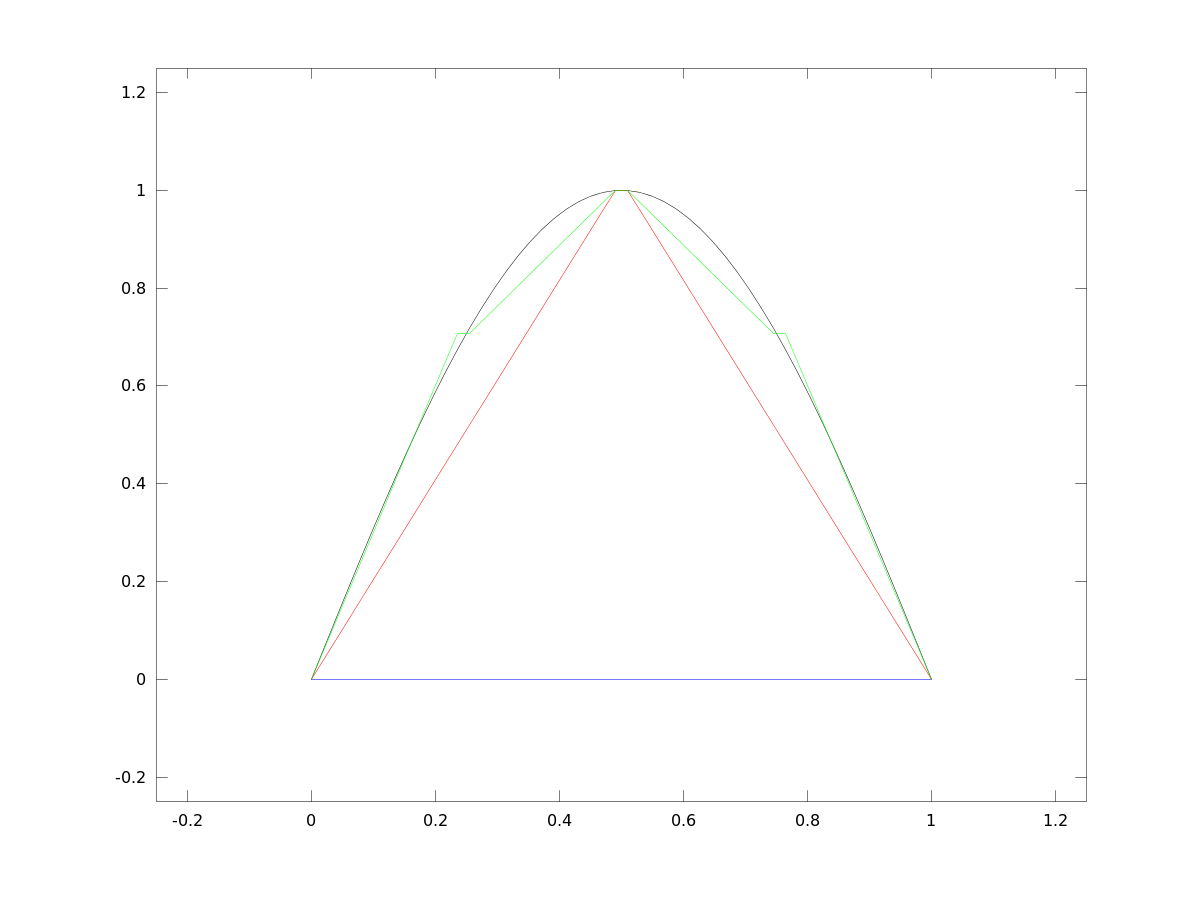
\includegraphics[scale=.17]{aplot.png}

The black line is $f(x) = \sin(\pi x)$ and may be a surface to be represented.
Simply calculating the distance between $f(0)$ and $f(1)$ yields a value of $0$, while if we chose more points between $0$ and $1$ and sum up the distances along this arch,
we improve the approximation to the distance along the curve.

Intuitively, we want a small distance in the $y$ space to mean that we don't have to go far along the curve to get between the points.
This is what would provide the accuracy up a given limit in the y-space.

Thus, a more complete approach of finding the distance between $f(x_1)$ and $f(x_2)$ would be use points between $x_1$ and $x_2$ and sum up all the distances along the way.
It is not completely clear how to select the points to fill in between $x_1$ and $x_2$ unless they happen to be of the form $x_1 + \alpha (x_2 - x_1)$.
I am guessing an accurate way to calculate the distance would be to compute 

$$\sum^N_{i=1}   |f(x_1 + \frac i N (x_2 - x_1)) - f(x_1 + \frac{i-1}{ N} (x_2 - x_1))| $$

for several values until it seems to converge (which it will if $f$ is continuous).
Choosing $N$ as powers of 2 would mean points could be reused, and there could be fancier ways of only increasing the precision (decreasing the distance between points) on sub intervals of the arch that
converge slowly.
However, this would require many function evaluations for simply computing the distance between two points.

Also, in higher dimensions it will be more complicated to find the distance between any two points because there may be arcs shorter than the one determined by a straight line between $x_1$ and $x_2$.


\section{First Version}

The first model has a fixed population size that is first formed from a random sample.
Then a selection of only the pareto points is conducted.
From then on, points are then added with evolutionary means.


Selection is done with a fitness-biased approach that randomly selects members of the population according to a distribution that favors the most fit.
This distribution is past in.
Another approach would be to use a truncation selection, where only the $k$ most fit individuals are crossed.

The original mutation is to add a delta to each component of the offspring from a uniform distribution.
Ideally the amount of mutation could decrease as points begin to converge (annealing).
The bounds of the uniform distribution are passed to the algorithm.

The fitness function for the initial model is to count the number of individuals that dominate any given point.
Additionally, a cost (passed in) is added to non-feasible points based on their distance to the closest feasible point.
This fitness function is somewhat costly, because it grows linearly with the population size (and involves sorting the distribution).
One approach to mitigate this cost presented in [citation here] is to conduct tournament cross over.
This involves sampling the population for $q$ points and selecting the most fit of these.
For the most part, individuals of the population are equally optimal for the MOP aside from the additional interests of genetic algorithm.
Because this algorithm does not focus new points in sparse regions of the representation, I doubt it would be harmed by using a tournament selection.

I will be comparing my algorithm with several other solvers, to see how well it performs.
The first and most simple solver to compare it against, is a simple random solver.
This solver samples the feasible region with a uniform distribution, and then returns those points of the resulting set that are non-dominated.

As a simple upgrade to this algorithm, I also implemented a random solver that iteratively moved the distribution towards the pareto set.
It does this by setting a generation size, and initially filling it with a random sample.
Then only the pareto points are selected, and new points are created by adding a uniform distribution to a random point from the previous generation.
This can be seen as a simplified version of the genetic algorithm in which case the crossover size is $1$ and which selection is not done after every crossover, 
but after an entire generation has been produced.
I will define this to be a generational feature of a genetic algorithm.

The generational feature could be very useful for speed improvements.
This is especially true when the selection process is costly.
Rather than always selecting the most fit individuals, the algorithm will assess the fitness every certain number of crossovers (say every $g$ crossovers).
Then the fitness of an individual at crossover $i$ is approximated by its fitness at crossover $i - (i $ mod $ g)$.
This means that offspring are unable to cross until they reach a certain maturity (the maturity has mean value $\frac g 2$).

Although this algorithm is a simplification of the genetic algorithm, it does have one unfair advantage to the genetic algorithm.
This is that each offspring $o$ has a only single parent $p$, so that there is a natural way to project infeasible points back on to the feasible region: simply scale the offspring back to the parent.
I did this by testing the feasibility of $o + (1 - 2^{-i})(p - o)$ with increasing $i=0,1,...$ until a feasible point is reached.
This assumes the bounds are easily evaluated in relation to the objective function.
If so, a similar approach would be possible for the genetic algorithm in convex problems by moving infeasible offspring towards
the center of its parents (the first moment of each parent).
Even in non-convex problems, this could be attempted and might work as long the algorithm is smart enough to not drive the power of $2$ too low when it doesn't produce a feasible point.

Finally, I will compare my solver to Matlab's.
In addition to comparing runtime performance, which may be language-related, I will also compare the representational quality of the pareto set.

Below are resulting computed points and pareto set for the random sampler, adaptive sampler, and genetic algorithm.
The goal is to minimize $f(x,y) = (x,y)$ subject to $y > (x-1)^2$ within the unit square.
The solvers were allow 500 evaluations.

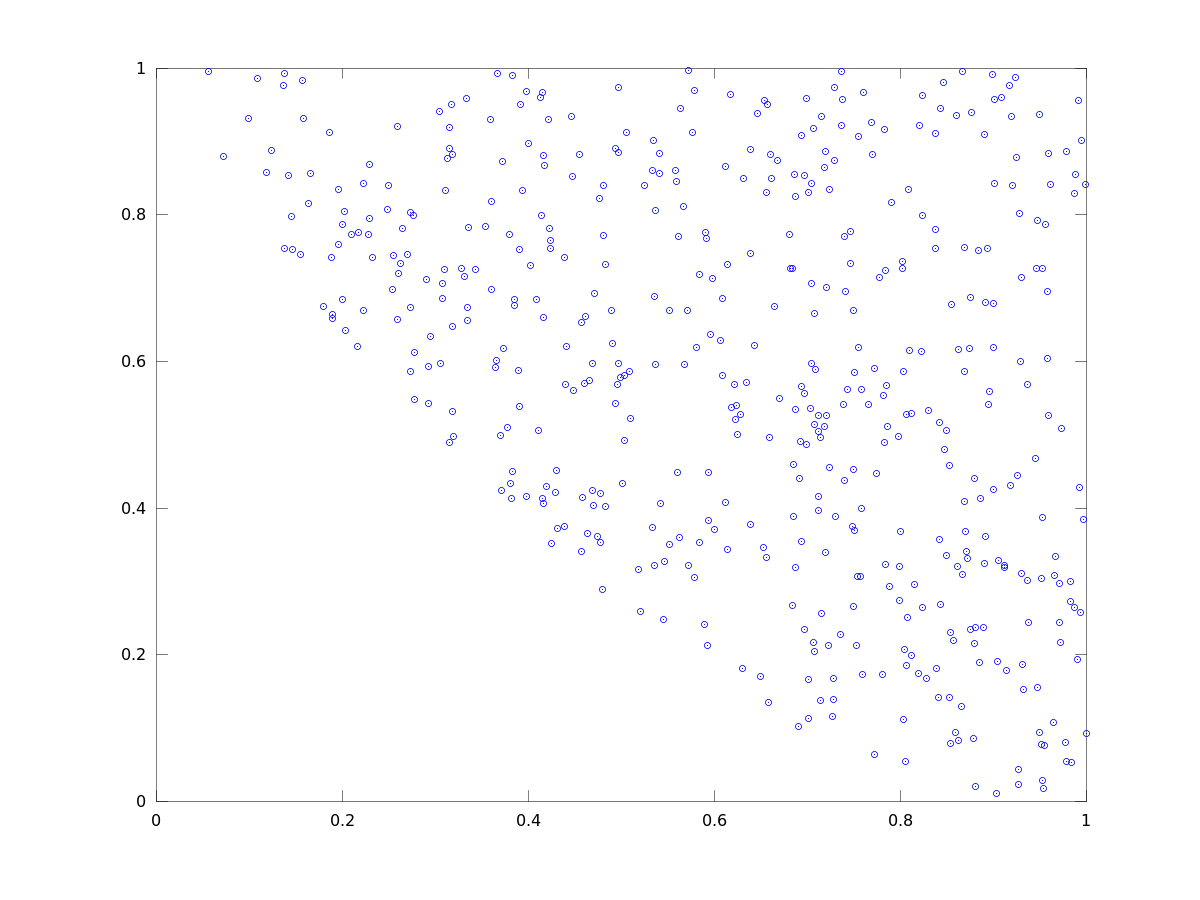
\includegraphics[scale=.1]{sampled_points.png}
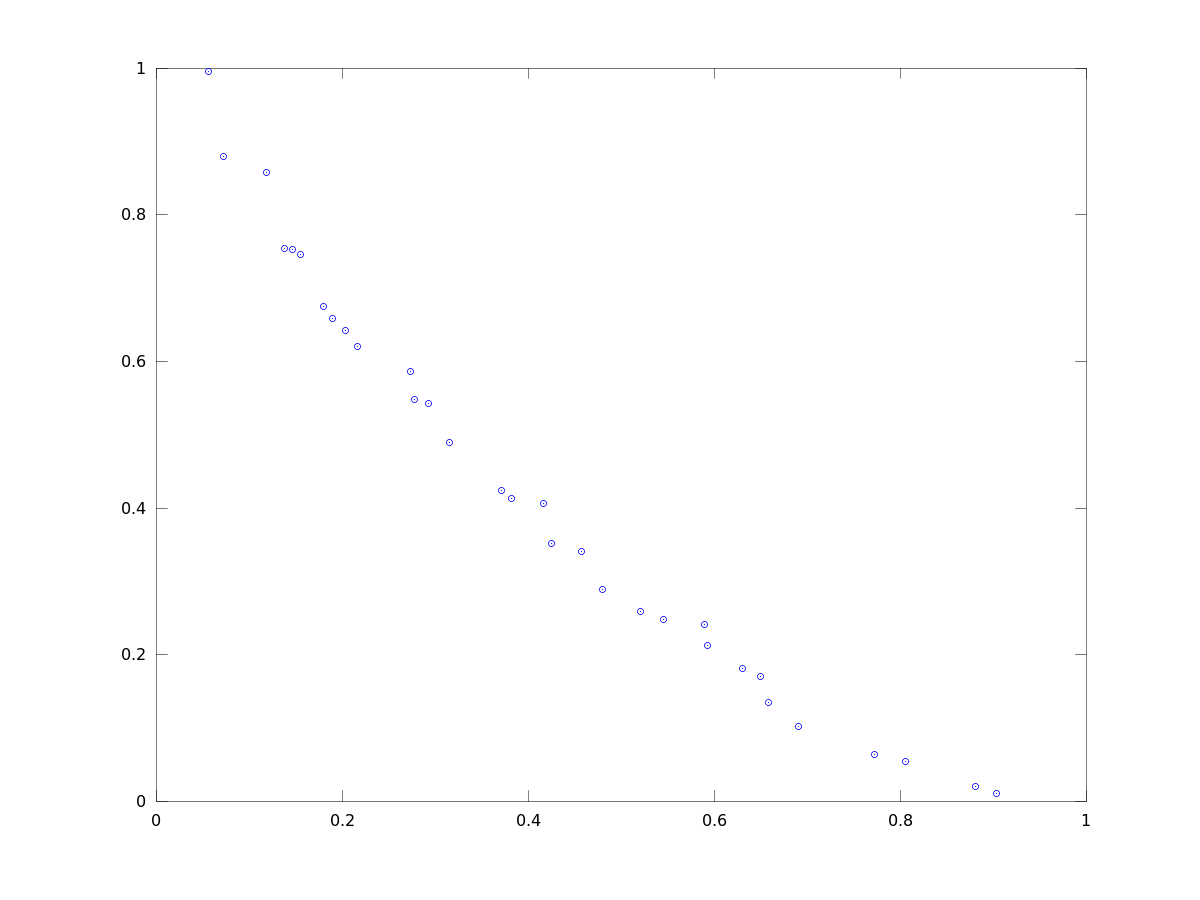
\includegraphics[scale=.1]{sampled_pareto.png}

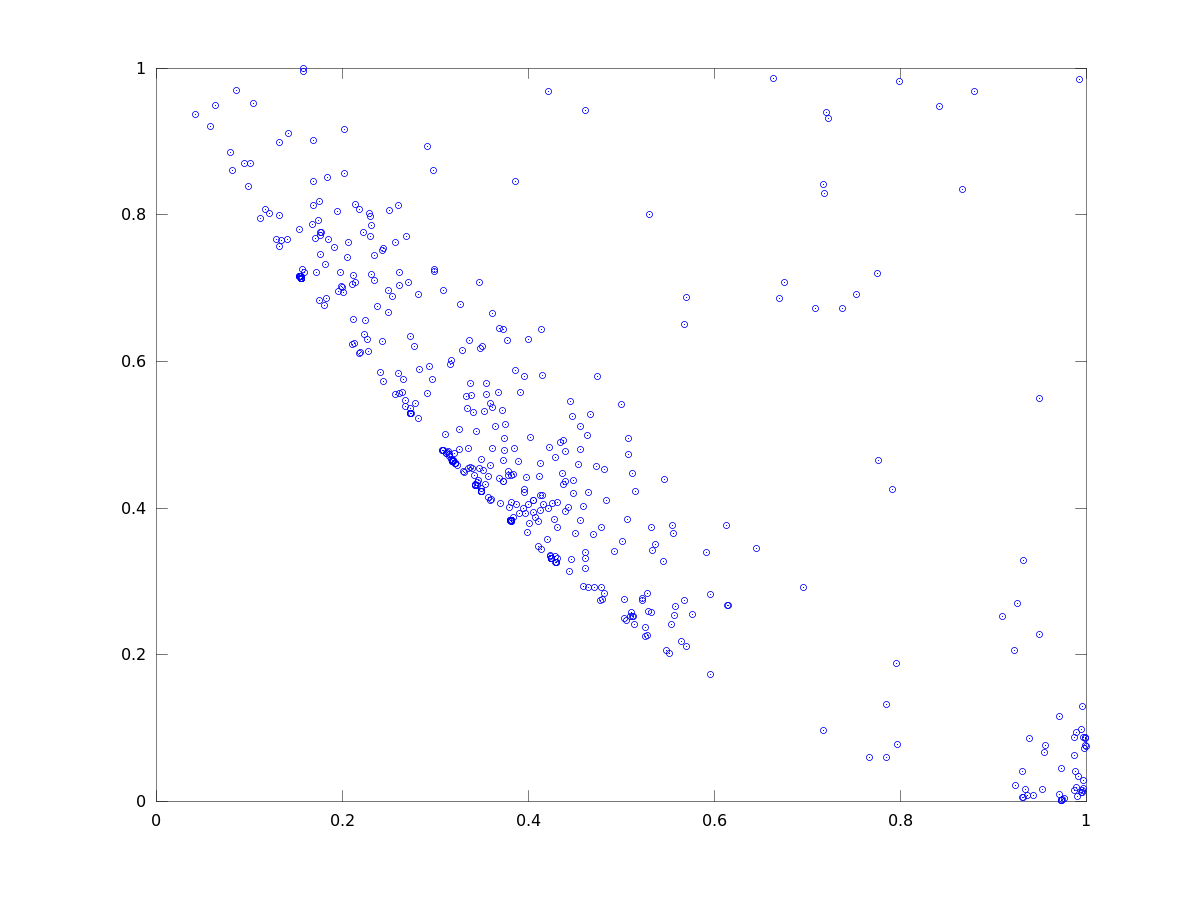
\includegraphics[scale=.1]{inc_points.png}
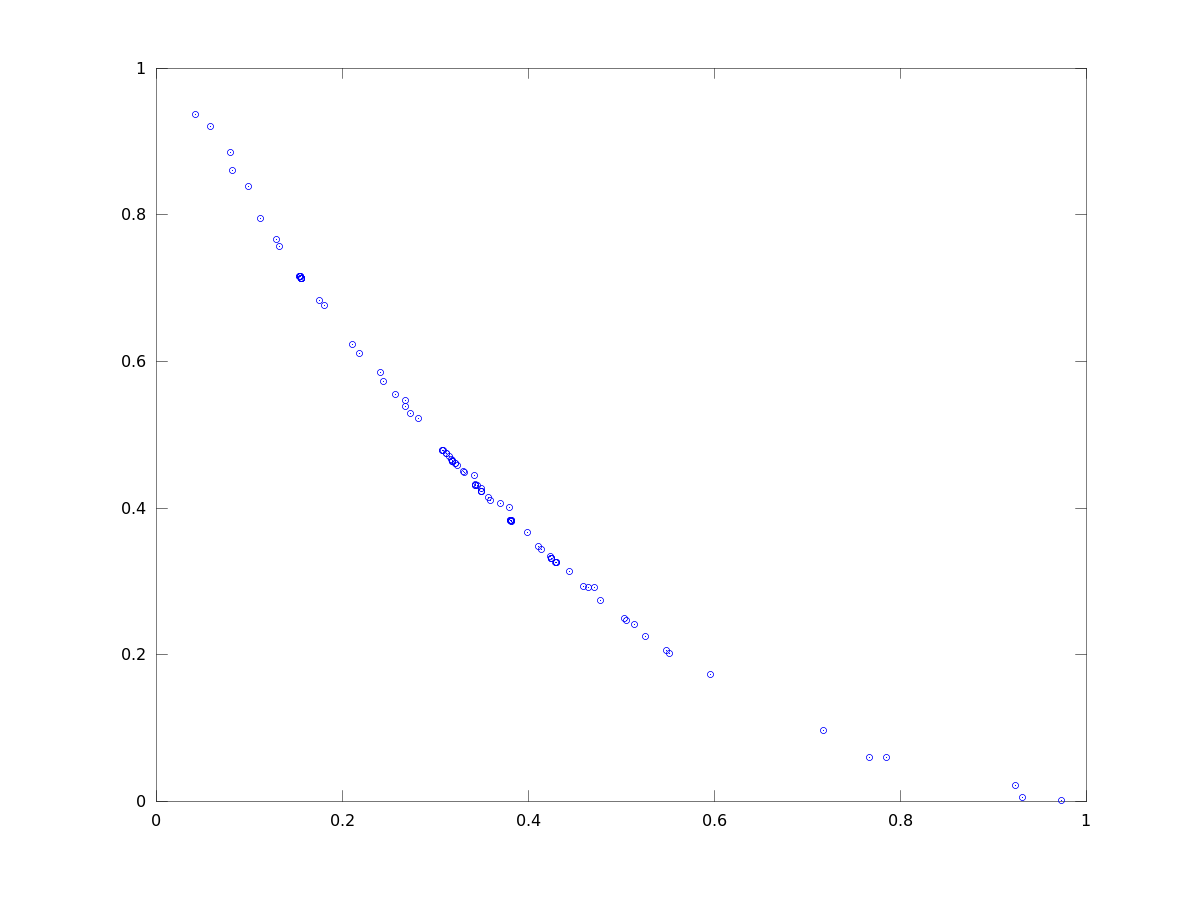
\includegraphics[scale=.1]{inc_pareto.png}

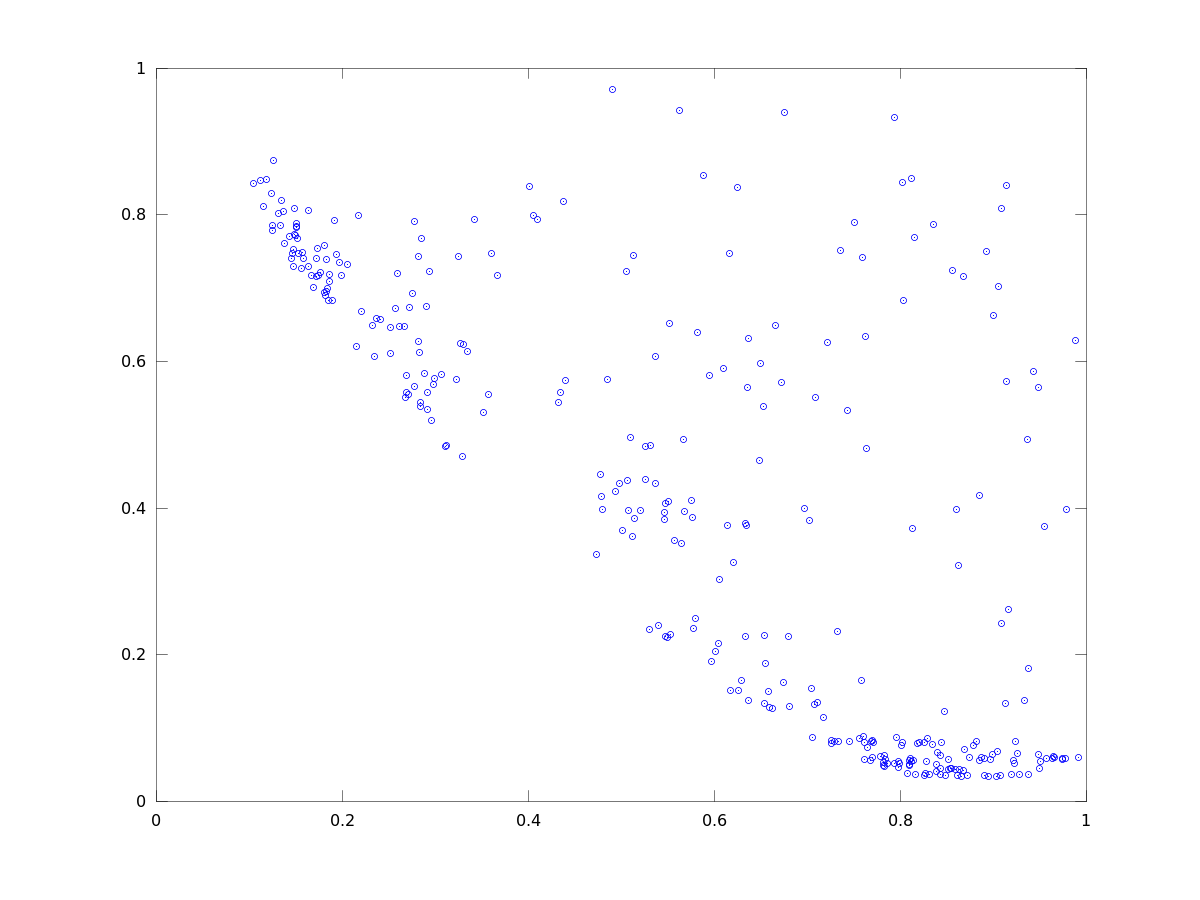
\includegraphics[scale=.1]{ga_points.png}
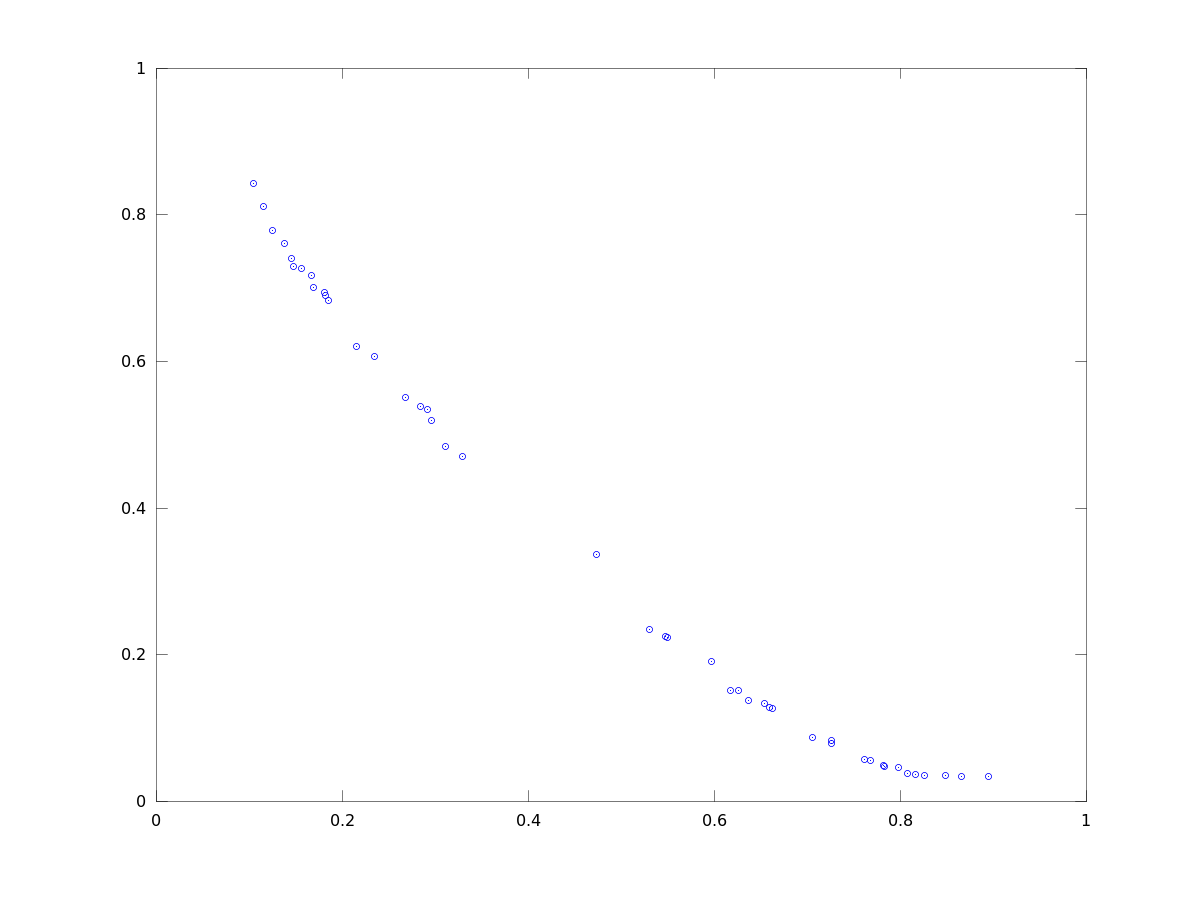
\includegraphics[scale=.1]{ga_pareto.png}

\subsection{Limitations and Future work}
The first genetic algorithm had several drawbacks.
By the time that random sampling has enough points to cover a pareto set, it has also likely created several points that are very near each other.
Because I also had no way of promoting diversification, the $y_N - y_I$ point generated had a high variance for values of $|S|$ that are otherwise reasonable.

As discussed in [citation here] this could be solved by using controlled elitism.
The first algorithm uses uncontrolled elitism in that it simply selects the most fit individuals to breed without considering their role in the population.
However, controlled elitism means that individuals are also selected based on how they contribute to the rest of the population.
Kalyanmoy and Tushar explain how this can be done to improve either exploitation, or exploration.

In the first genetic algorithm I wrote, I needed to keep a reserve population, so that I could be sure the distance to the nearest feasible point is well defined.
This may motivate keeping other sub populations.


On initial, simple problem sets, the first algorithm seems to work best with a crossover size of 2, a very high cost to infeasible points, and a highly preferential fitness function
(highly preferential means a distribution for selecting individuals set by $\frac{-fitness }{ -\max(fitness))^5}$  ).
Under these conditions, we see that the most useful evolutionary instrument is the mutation, as opposed to crossover.
I conjecture that this is because crossing pareto optimal points from distant x-points does not likely produce another optimal point.
With a small crossover size, and a very selective fitness function, sometimes a point is crossed with itself (The selection distribution does not contain replacement.)

This suggests that introducing \emph{incest} may improve the crossover process.
Incest is a measure of how close individuals who are crossed are to each other.
For example, with a crossover size of $2$, we could define the incest used by a genetic algorithm to be 
the average of all distances between crossed individuals throughout the algorithm.
This will improve the algorithms exploitation of individuals, but not help its exploration.

Rather than using an initial random sample, I could try to only use a small population in the beginning and simply applying the same evolutionary principles from the start.
This would mean that less function evaluations are used at the beginning in order to get the algorithm started.
However, the algorithm would need to start out with an emphasis on mutation in order avoid getting stuck in the nearest pareto region.
Also, it may be efficient to treat individuals as leaves of the $n$-dimensional Qaudtree used to represent the outcome space [more about how the quadtrees can improve the efficiency].
This may encourage the points to be more equally spaced from the start, because new points are not just randomly mutated, but are randomly 
selected at a certain depth (aka distance) from their parents based on how dense the representation is in that area.
This would make implementing a multi-stage exploration/exploitation algorithm easier.
This would work by first exploring the outcome space until exploration doesn't seem to be finding more unrelated points.
Then the algorithm would begin to exploit the pareto solutions it has already found in order to find the best representation.



\end{document}

%breed -> crossover


